% !TEX root =single_chapter_dalek.tex
\chapter{Automatic fitting of Type~Ia~Supernova~spectra}
\label{chap:dalek}
\section{Introduction}
\label{sec:dalek_intro}

The last chapters (Chapters \ref{chap:sn1572_starg, chap:sn1572_hires, chap:sn1006_flames}) were dedicated to the hunt for donor stars and did not use the measurements from the \sneia\ themselves. In this chapter we will describe the extraction of nucleosynthetic yields and energies from optical spectra as well as the automation of this process.

The main sources of information in spectra are the shape/strength of the spectral features and their evolution with time. There have been a few attempts to extract the details of the stellar explosions from one or both of these sources. All of them employ the technique of fitting the observations using synthetic spectra. A critical part of this process is the radiative transfer algorithm used to generate the synthetic spectra, which has been implemented in several different codes.


\cite{2000PhDT.........6F} wrote a very simple radiative transfer code called \synow. \synow\ is a highly parametrized code and thus is mainly used for line identification rather than actual fitting of \snia\ spectra. 
The main code used in this work is a further development of the code described in \citet{1993A&A...279..447M}  and \citet{2000A&A...363..705M}, henceforth named the \gls{mlc}. Compared to the \synow\ code the \gls{mlc} code calculates a \gls{radeq} temperature and uses this to compute internally consistent ionization ratios. In addition, \gls{mlc} takes electron scattering into account as well as allowing for non-resonance line scattering. 

Codes such as PHOENIX \cite{1999JCoAM.109...41H}, SEDONA \cite{2006ApJ...651..366K} and ARTIS \cite{2009MNRAS.398.1809K} are powerful 3D radiative transfer codes. They are the most `physical' codes available but take hours to days on supercomputers to produce spectra. As they take a considerable amount of time and computational power, these codes, however, are not practical for fitting many observed spectra.

 \cite{2007Sci...315..825M} showed that the brightness of a supernova relies mainly on the production of \Ni. Faint \sneia\ (\gls{91bg}) produce roughly 0.2\,\msun of \Ni. Most \sneia\ produce roughly 0.6\,\msun, with some luminous \sneia\ (\gls{91t}) producing up to 0.9\,\msun. All luminosity types enclose approximately 1\,\msun\ of ash. This remarkable find was made by manually fitting 23 \sneia\ using the \gls{mlc}. There are however many more spectroscopically well sampled \sneia\ and soon there will be even more observed expected from the next generation supernova searches. Such large datasets cannot be effectively studied with manual fitting techniques. An automated procedure can not only fit many supernovae but will also explore the parameter space to calculate error estimates. Strict quality measures necessary for an automatic fitter can also help when interpreting physical quantities generated by the code. We present an automated way of fitting supernovae using the  \gls{mlc} (in collaboration with Stephan Hachinger and Paolo Mazzali).

In section \ref{sec:mlc_intro} we will introduce the inner workings of the \gls{mlc}-code.  We will discuss the properties of the parameter space on one example fit in Section \ref{sec:manual_sneia}. Section \ref{sec:ga_brief_intro} provides an introduction to \gls{ga}, which are the optimization strategies of choice in the automatization of the \gls{mlc}.  We will present the current implementation of the autofitting code in Section \ref{sec:geneticdalek} (\gls{dalek}).  Finally we will conclude and give an outlook over future work of this project in Section \ref{sec:dalek_conclusion}.

\section{The \glsentryname{mlc} Code}
\label{sec:mlc_intro}

The \gls{mlc} code, used in this work, is described in detail in \citet{2000A&A...363..705M} and we will give only a very short introduction to the key concepts here. We refer the reader to \citet{2000A&A...363..705M} for a more detailed description of the code. A more advanced version, using abundance stratification, but not used in this work  is described in \citet{2000A&A...363..705M}. 

Based on spectra, the phase of the evolution of a supernova can be divided into the photospheric phase and the nebular phase. The \gls{mlc} only creates synthetic spectra for \snia\ in the photospheric phase. In the photospheric phase the supernova can be approximated by a sharp photosphere emitting a black-body spectrum with a fast moving ejecta-layer on top.

\subsection{Radiative Transfer}
Radiative transfer calculations attempt to provide the wavelength dependent flux emerging from the atmosphere for a given input boundary condition at the base of the atmosphere. Computing the attenuation for the given input flux ($F_0$) is a critical part of this process. This wavelength-dependant attenuation factor is called the opacity $\tau$:
\begin{equation}
\label{eq:rad_trans}
	F(\lambda) = F_0(\lambda)\,e^{-\tau(\lambda)},
\end{equation}
where $F$ is the observed flux and $F_0$ is an assumed distribution of input flux before being absorbed by the plasma, which imposes the attenuation factor $e^{-\tau}$.
There are many physical processes relevant to supernova radiative transfer. The line opacity (bound-bound transitions) has the biggest impact on the final spectrum. The lines in \snia\ spectra are the prime indicators for elemental abundance. In contrast to lines, which occur at one specific frequency, \gls{thompsonscat} is independent of frequency and only depends on the state of the atmosphere. \gls{thompsonscat} is an important way to redistribute photons in angular space (i.e. making the radiation field more isotropic) and thus also has a strong influence on radiative heating/ionization of the plasma. Other sources of opacity like free-free absorption and bound-free absorption are thought of as second order effects and are not implemented in the \gls{mlc}. As the \gls{mlc} is required to be fast only bound-bound opacity and \gls{thompsonscat} is implemented in the code.

Unlike stellar atmospheres, in supernova ejecta one needs to consider the photon's Doppler shift in relation to the surrounding medium. One major assumption that the code makes is the so-called \gls{sobolevapprox}. The \gls{sobolevapprox} assumes that lines have only a single frequency at which they can be excited  (no natural, thermal or other line broadening), This assumptions is a good approximation where photons are moving through a medium where the velocity gradient is so high that they are only in resonance with one line (no blending) in a very small region. This \gls{sobolevapprox} is one important factor of making the code fast yet still reproducing the observed spectra rather well.

In addition the \gls{mlc} assumes the ejecta to be in homologous expansion. This means that the velocity is a linear function of the radius:
\[
	v=  r / t.
\]

Combining both the Sobolev approximation with the assumption of homologous expansion yields this relatively simple formula for line opacities:
\begin{equation}
\label{eq:sobolevapprox}
\tau_{lu} = \frac{\pi e^2}{m_e c}\, f \lambda t_{\rm exp} n_l\, \left(1 - \frac{g_l n_u}{g_u n_l}\right), 
\end{equation}
where $\tau_{lu}$ denotes the opacity going from the lower state to the upper state of an atom, $e$ is the electron charge, $m_e$ is the electron mass, $f$ is the absorption oscillator strength of the line, $\lambda$ denotes the wavelength, $t_\textrm{exp}$ the time since explosion, $n_x$ the number of atoms in the state $x$ and $g_x$ is the statistical weight of the state $x$.

Although producing relatively good synthetic spectra, the assumptions of homologous expansion and \gls{sobolevapprox} have their caveats. In the case of homologous expansion it is thought to be a very good approximations after the first few minutes of the explosion, but maybe effected when, for example, the ejecta interacts with surrounding material. The main caveat for \gls{sobolevapprox} is that a line is not a delta-function, as assumed in the \gls{sobolevapprox}. If two strong lines are close in frequency space it can lead to the first line shielding the second line. Despite these caveats, however, the \gls{sobolevapprox} and homologous expansion are widely used and have been demonstrated to provide an adequate compromise between accuracy and computational practicality for fitting the spectra of supernova ejecta.

We have discussed the propagation of the photons in the plasma but have not discussed the state of the plasma yet. The simplest assumption for the state one can make is \gls{lte}. In this case the Boltzmann formula describes the level populations in a single ion:
\[
\frac{n_j}{n_{\rm ground}} = \frac{g_j}{g_{\rm ground}}\,e^{-(\epsilon_j - \epsilon_{\rm ground})/kT},
\]
where $n_j$ is the population of the $j$-th state of the atom, $g_j$ is the statistical weight of the $j$-th state, $\epsilon_j$ is the energy of the $j$-th state and $T$ is the temperature of the plasma.
Similarly we can calculate the ionization state using the Saha-equation:
\[
	\frac{N_j}{N_{j+1}} = n_e \frac{U_j(T)}{U_{j+1}(T)}\,C_I T^{-3/2} e^{\chi/kT},
\]
where $N_x$ are the total ion population with ionization state $x$, $U_x$ is the partition function for the ionization state $x$, $n_e$ is the number density of electrons, $C_I$ is a universal constant and all other symbols have their usual meaning. 


In the \gls{nebularapprox} we approximate the radiation field by a diluted black body:
\[
J = W B(T_R),
\]
where $J$ is the mean intensity, $T_R$ is the radiation temperature and $W$ is the dilution factor. In the standard \gls{nebularapprox} $W$ differs from 1.0 due to purely geometrical reasons: the photon count falls with distance to the source ($1/r^2$ for a point source). For an extended source the geometric part of the dilution factor takes the following form \citep{1978stat.book.....M}:
\begin{equation}
W(r) = \frac{1}{2}\left[1-\sqrt{1-\left(\frac{r_\textrm{ph}}{r}\right)^2}\right]
\label{eq:dilution}
\end{equation}
This concept can be generalised to a \gls{modnebularapprox} where the effects of attenuation and scattering (e.g. line and \gls{thompsonscat}) on $W$ can also be included. Using $W$ and $J$ and assuming \gls{lte} one can easily calculate the electronic and ionization states of the plasma:
\[
\frac{n_j}{n_{\rm ground}} = W \left( \frac{n_j}{n_{\rm ground}} \right) _{T_R}^{\rm LTE}
\]
and 
\[
\frac{N_j}{N_{j+1}n_e} = W \left( \frac{N_j}{N_{j+1}n_e} \right) _{T_R}^{\rm LTE}.
\]
This simple form of the \gls{nebularapprox} only considers radiative excitation/de-excitation and ionization/recombination from and to the ground state, but has the advantage of solving the state of the plasma computationally inexpensively.
The \gls{mlc} uses a variant of the \gls{modnebularapprox} which includes radiative excitation/de-excitation from excited states and a different treatment of the \gls{uv} radiation field (which contains most ionization edges). For a detailed description of the modifications please refer to \citet{1993A&A...279..447M} and references therein. 

In the \gls{mlc} code the two fundamental properties of the radiation field - temperature and the dilution factor - are determined from a \gls{mc} simulation. We first measure the mean frequency of the photons and bolometric intensity. We then infer the temperature by requiring the black body to have the same mean frequency (Wien approximation). The dilution factor can then be fitted to match the bolometric intensity. We note that close to the photosphere the dilution factor is influenced mainly by the geometry and should be close to 0.5 (see Equation \ref{eq:dilution} for $r=r_\textrm{ph}$). As the \gls{mc} process is statistical and the dilution factor an approximation this might vary, but we assume this to be still an important factor to determine if the model is realistic. 

In summary, the approximations described in this section make the \gls{mlc} fast, yet still providing an acceptable representation of reality. This makes the \gls{mlc} code feasible to use for modelling data. 

\subsection{Monte Carlo Radiative Transfer}

We have so far only described the approximations made by the code, but not how these are implemented and work together. In this section we will give an overview of the process and design of the \gls{mlc} code.

First the ejecta in the \gls{mlc} is divided into 20 concentric shells with an equal thickness in $1/r$, where r is the radius from the centre of the explosion. Each shell has a uniform density which is drawn from the well known empirical \gls{w7}. The \gls{mlc} also allows the change of this density structure, but for all this work we have kept the \gls{w7} density structure. In addition, we assume a homogenous abundance distribution throughout the whole model. There is, however a \textit{stratified} version of the code that allows for different abundances in each shell. We have opted to use the simple homogeneous version as the parameter space is very complex even for this homogeneous version. We plan to extend the automatic fitting procedure to use the stratified version at a later date. In addition, we calculate the time since explosion $t_\textrm{exp}$ using the time of the photometric maximum and adpopting a rise time estimate of 19.5 days. The photospheric velocity \gls{vph}, the bolometric luminosity \gls{lbol} and abundances for the chosen elements are the input parameters to the \gls{mlc}. 

To conserve \gls{radeq} the \gls{mlc} uses photon packets instead of individual photons. Each photon packet, described by  frequency and number of photons, contains the same energy (more photons per packet in the red than in the blue). For pure elastic scattering events - the absorption frequency is the same as the reemission frequency - the number of photons is conserved in each packet. For line absorptions this is generally not the case. The \gls{mlc} allows for photon branching, which means that the photon can be emitted in a different transition than it was absorbed in. Once absorbed the new emission transition is chosen by a weighted random process \citep[for a more details see][]{2000A&A...363..705M}. The number of photons in the packet is adjusted to conserve the co-moving energy of the packet, thus preserving the energy between matter and radiation field (\gls{radeq}).


The \gls{mc} simulation begins by calculating the plasma condition using an initial guess of temperature and dilution factor for each shell. A photon packet is emitted with a random frequency and a random angle drawn from a blackbody distribution.  An event optical depth is calculated from a uniform random distribution so that $\tau_\textrm{event}=-ln(z),\ z \in (0,1]$ (follows from sampling the Equation \ref{eq:rad_trans}).  There are three possible outcomes for the photon in each Monte Carlo step. First we calculate the length of the path ($s_e$) that the packet can travel freely before $\tau_{\rm event}$ is equal to the Thompson scattering opacity $\tau_{\rm event} = \sigma_\textrm{T} n_e s_e$. Secondly we calculate the same path length for the lines $s_l$ using as a target opacity $\tau_e + \tau_\textrm{line}$ for line scattering (where $\tau_e=\sigma_\textrm{T} n_e s_l$ and $\tau_\textrm{line}$ is the line opacity calculated with Equation \ref{eq:sobolevapprox}). If $s_e$ is the shortest then \gls{thompsonscat} occurs and the photon is assigned a new direction and a new $\tau_\textrm{event}$ is drawn and we start anew.  If $s_e<s_l<s_\textrm{exit}$, where $s_\textrm{exit}$ is the length to exit the shell, line scattering occurs and the photon is absorbed by an atom. This excited atom can then de-excite through many lines. \gls{mlc} randomly chooses a downward transition for the whole packet (taking the appropriate weights into account) and adjusts the photon number in the packet to ensure \gls{radeq}.  Finally, if both paths are longer than the path to exit the current shell, then the photon exits the current zone and a new \gls{mc} step begins.This process is iterated until either the photon packet escapes the outermost shell - in which case the photon number and frequency is recorded - or penetrates the photosphere in which case the photon is discarded and a new one drawn. 

This iterative process is first used in the \gls{mlc} code to prepare the plasma state. In this initial simulation each packet status is recorded at the mid-point of each shell. This information is used to calculate a new temperature and dilution factor which then leads to updated plasma conditions (level populations and ionizations). This procedure is repeated until the plasma temperature converges. Once convergence is reached the actual Monte-Carlo simulation begins. 

The final spectrum is not calculated using the number and frequency of the escaping photon packets. Instead we use the photon packets to estimate the source function as a function of wavelength and then calculate the emerging spectrum using a formal integral solution of the radiative transfer equation \citep[a more detailed description of this method in][]{2000A&A...363..705M}. This has the advantage of reducing noise in the spectrum due to \gls{mc} noise. 

In summary, the \gls{mlc} produces realistic spectra in a competitive calculation time (one spectrum per minute on a modern computer). A more detailed description of the code can be found in  \citet{1993A&A...279..447M} and \citet{2000A&A...363..705M}. There is a abundance stratified version of the \gls{mlc} code, which has not been described in this work but can be reviewed in \citet{2005MNRAS.360.1231S}.


\section{Manually fitting a Type Ia supernova}
\label{sec:manual_sneia}

We extract physical quantities from the \snia\ spectra by adjusting the parameters of the \gls{mlc} until the code produces a similar synthetic spectrum to the observed one. For now this fitting process for \sneia\ is an arduous manual task, which requires detailed knowledge about the inner workings of the \gls{mlc} and its approximations. Known problems, like the excess in the \gls{nir} (described in more detail later) and the high velocity calcium, necessitate one to prioritize between different quality measures. This also leads to a subjective `best-fit', although experts in \gls{mlc} fitting seem to come to the same conclusion despite their different approaches. We will first illustrate this fitting process on one example - \sn{2002}{bo} 10 days before maximum \citep{2004MNRAS.348..261B} - which has been fitted manually by \citet[][]{hachinger_dipl2007}, before moving to our automatic optimization attempts in Section \ref{sec:dalek}. 
\begin{figure}[htbp] %  figure placement: here, top, bottom, or page
   \centering
   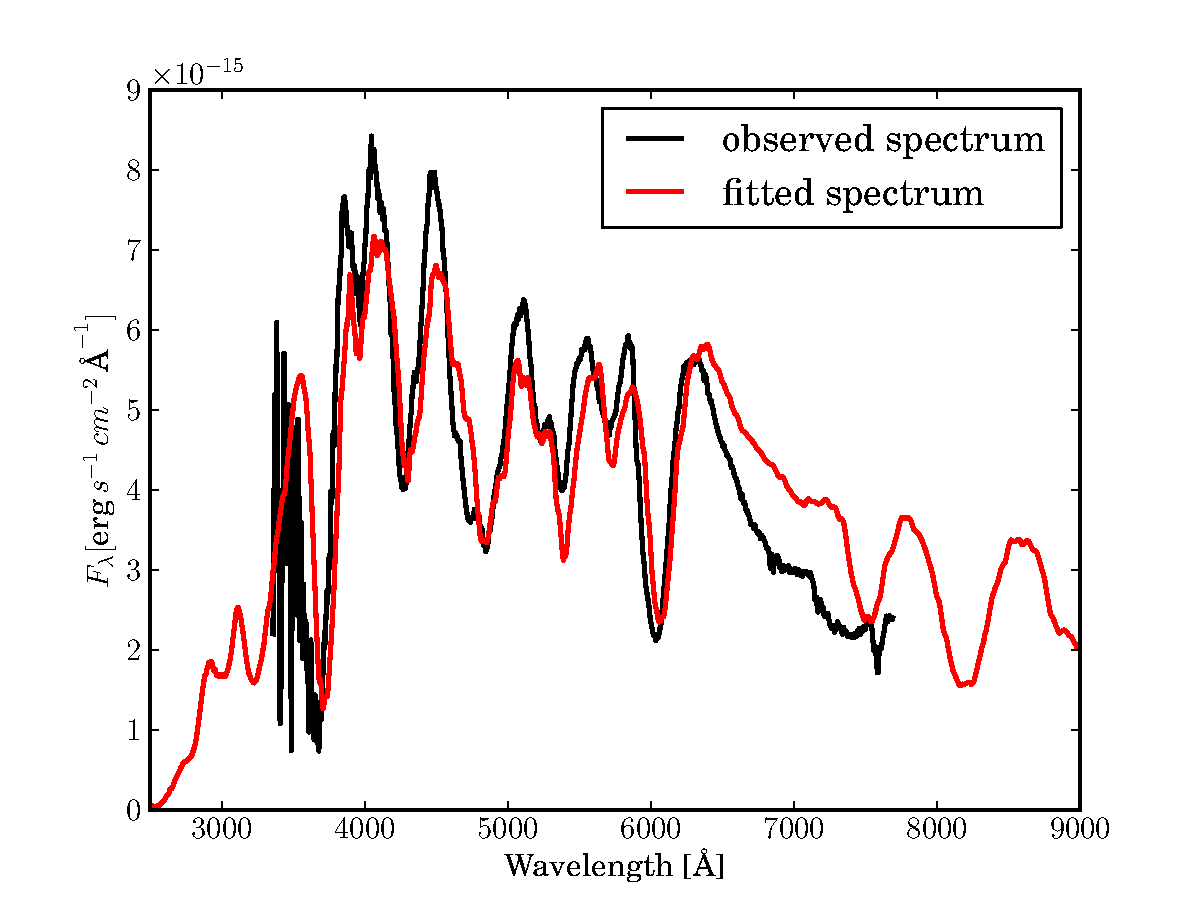
\includegraphics[width=0.7\textwidth]{chapter_dalek/plots/bf2002bo-10.pdf} 
   \caption[Spectrum on SN 2002bo with MLMC fit]{Spectrum of \sn{2002}{bo} \citep{2004MNRAS.348..261B} with \glsentryname{mlc} fit by \citet{hachinger_dipl2007}. The excess in redwards of 6500\,\AA\ is a common problematic features of these fits.}
   \label{fig:sn2002bo-10_bf}
\end{figure}

The first step in any fitting procedure is to initialize the parameters. The luminosity distance, redshift and time since explosion \gls{texp} are initialized from data available on the supernova and are not fitted with the \gls{mlc} code. The initial choice of luminosity and photospheric velocity is based empirically on photometry and \gls{texp}. When manually fitting the spectrum we only consider contributions from the elements listed in Table \ref{tab:2002bo_bestfit_abundances}. When initializing these for a manually fitting procedure we use empirical data (this procedure is described in detail in Section \ref{sec:dalek}). In the fitting process several elements are treated specially. The abundance of \Ni\, for example, is given as the abundance of initial nickel synthesized in the explosion. Since \Ni\ is unstable this unified mass of \Ni\ will decay first to \Co\ which then decays to \Fe. This decay is accounted for (i.e. the abundances of \Ni, \Co\ and \Fe\ are calculated from the initial \Ni\ mass and \gls{texp}). In all further discussions, cobalt will always refer to radioactive \Co, the daughter of \Ni\ (we do not consider any stable isotopes of cobalt that may have been synthesized in the explosion). The \Fe\ abundance is determined by adding the \Fe\ obtained from the \Ni\ decay to the iron and pre-exisiting \Fe\ (Fe$_0$). In addition we lock the ratio of titanium and chromium as we do believe this to be degenerate in the fit. 

explosive nucleosynthesis reference \citep[e.g.][]{1999ApJS..125..439I}

\begin{figure}[tb] %  figure placement: here, top, bottom, or page
   \centering
   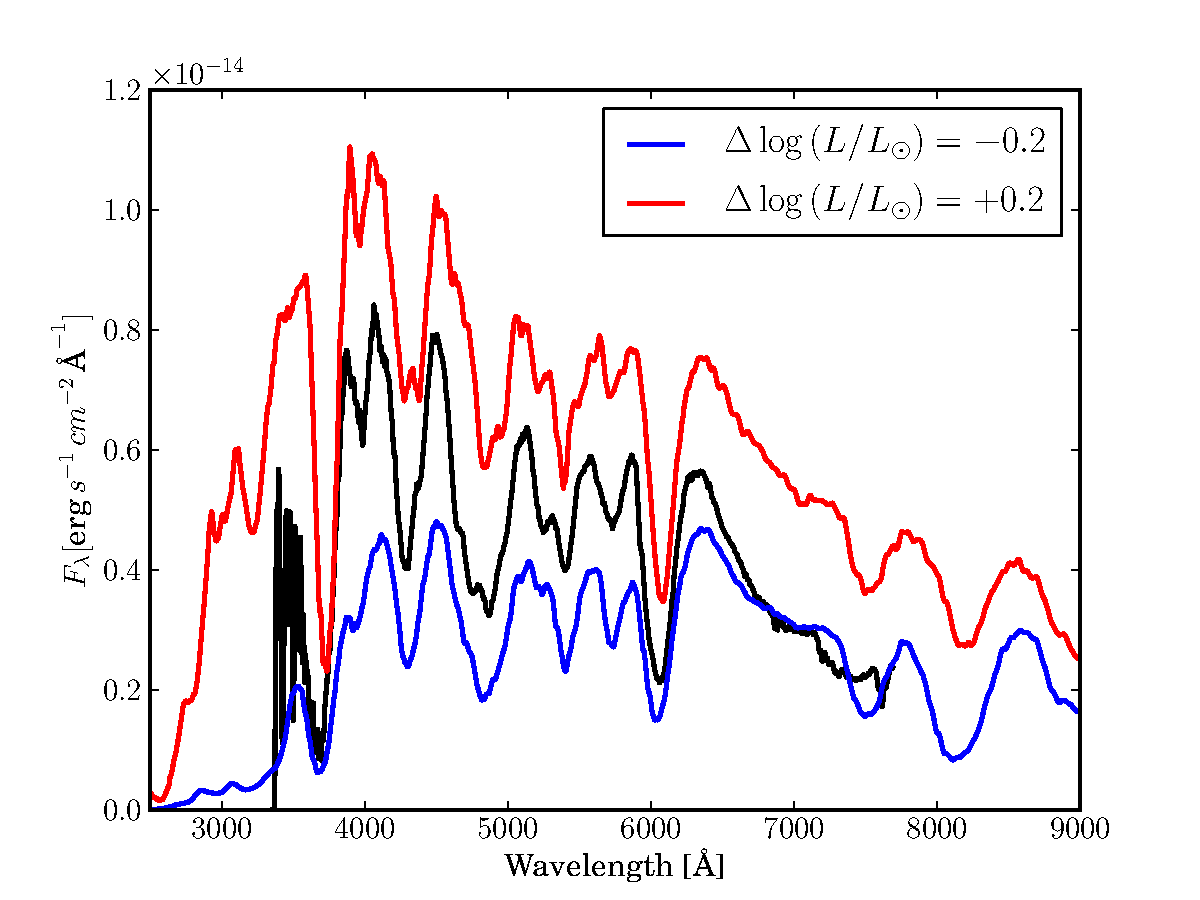
\includegraphics[width=0.7\textwidth]{chapter_dalek/plots/bf2002bo-10_lum.pdf} 
   \caption[Effect of luminosity on MLMC fit]{We have perturbed the luminosity around the best fit value. The most noticeable effect is the continuum offset. There is also a slight change in the overall slope of the spectrum.} 
   \label{fig:sn2002bo_lum_offset}
\end{figure}

Next we will describe the unique impact each parameter has on the spectrum and how that is used to arrive at a best fit. There are three main parameters that have the most influence on the overall spectrum fit: Luminosity, photospheric velocity and abundance in \gls{ige}.
A large offset in \lum, relative to the best fit parameter, is easily visible as a large offset of the continuum (see Figure \ref{fig:sn2002bo_lum_offset}). Thus it is easy to constrain the parameter space in \lum. \lum\ also has influence on the temperature of the model through:
\[
L_{\rm bol} = 4\pi\sigma\, R^2\,\teff^4 = 4\pi\sigma(\gls{vph}\gls{texp})^2 \teff^4,
\label{eq:lum_temp_relation}
\]
where \gls{teff} can be calculated by the model parameters \lum\ and \gls{vph}. 

Velocity in astronomy is often measured using the Doppler shift of atomic lines. In this case however it is hard to measure \gls{vph} from atomic lines.  Lines are created at different depths and thus at different velocities. This smears out the line profiles which makes fitting velocities nearly impossible using this technique. The main impact of photospheric velocity is establishing the temperature structure with the given luminosity. A model with a too high photospheric velocity will have expanded more than the observed spectrum and thus will be cooler. This results in a spectrum that is too luminous in the red and not luminous enough in the blue (see Figure \ref{fig:sn2002bo_vph_offset}). A secondary effect is that the ionization state will be wrong (blue radiation field will lead to more photoionization and vice versa), which can be seen in various lines. 


\begin{figure}[tb] %  figure placement: here, top, bottom, or page
   \centering
   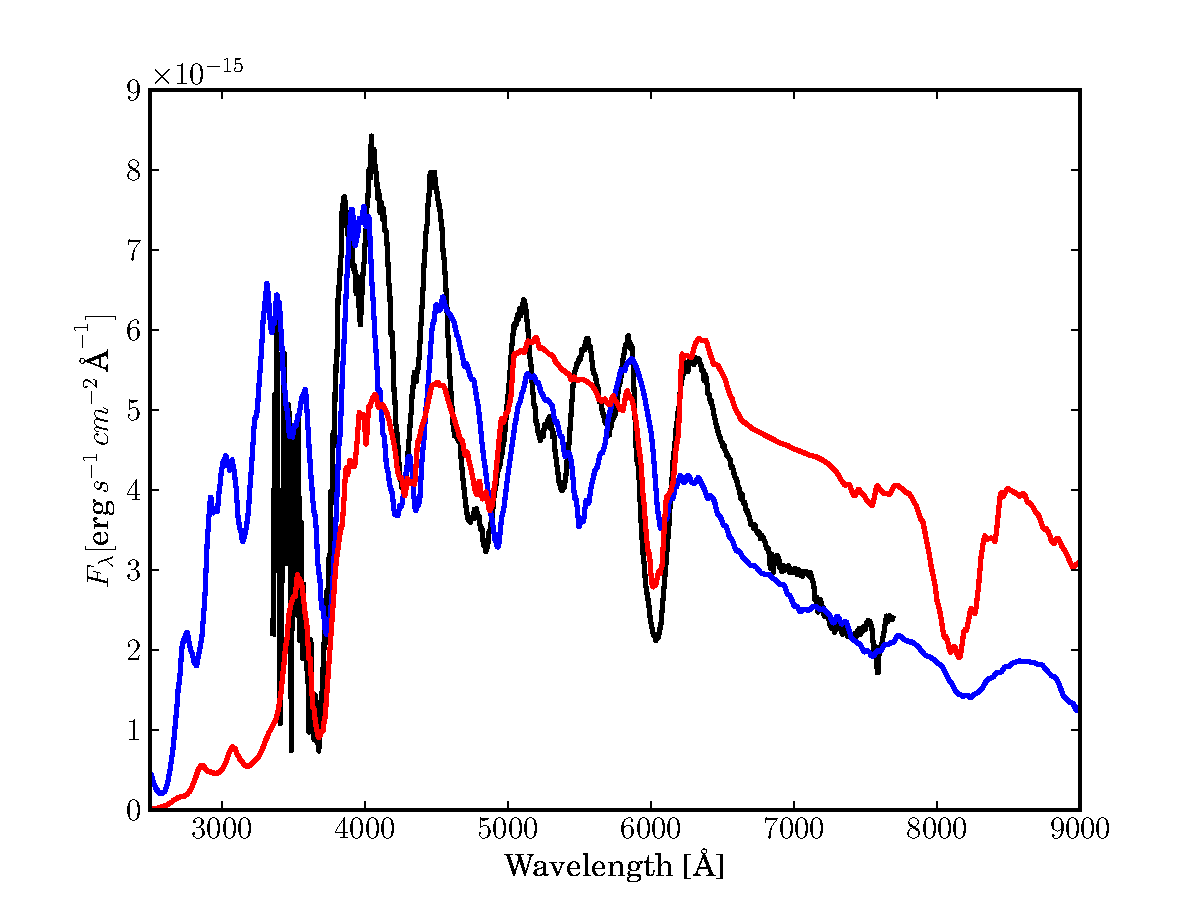
\includegraphics[width=0.7\textwidth]{chapter_dalek/plots/bf2002bo-10_vph.pdf} 
   \caption[Effect of photospheric velocity on MLMC fit]{The photospheric velocity has been perturbed around the bestfit. If the velocity is too small, the spectrum is too blue and vice versa.}
   \label{fig:sn2002bo_vph_offset}
\end{figure}


The \gls{ige} have a similar influence on the overall flux distribution as the photospheric velocity. 
We assume, as discussed previously, no stable cobalt. All \gls{ige} elements reprocess the flux heavily by absorbing bluewards of $\approx 3800\,\AA$ and fluoresce in the red part of the spectrum. For example, a too high abundance will suppress the flux in the blue too much and will cause the spectrum to be over-luminous in the red (see Figure \ref{fig:sn2002_ige_offset}). Although physically different from the photospheric velocity, phenomenologically these are similar. The degeneracy is broken by identifiable iron lines in the spectrum as well as the ionization balance determined by the temperature (mainly influenced by photospheric velocity and luminosity). This near degeneracy causes a very complex parameter space. The titanium/chromium abundance ratio is fixed and only one of these elements is fit. Like $Ni_0$ and $Fe_0$, titanium and chromium provide strong flux suppression in the blue and fluoresce in the red. Chromium can be partly constrained due to a blended line just blueward of the \gls{uv} calcium feature, but other than that we believe them to be slightly degenerate with the other \gls{ige}. We disregard the elements scandium, vanadium and  manganese as they seem to have little influence on the spectrum at their predicted abundances.

\begin{figure}[tb] %  figure placement: here, top, bottom, or page
   \centering
   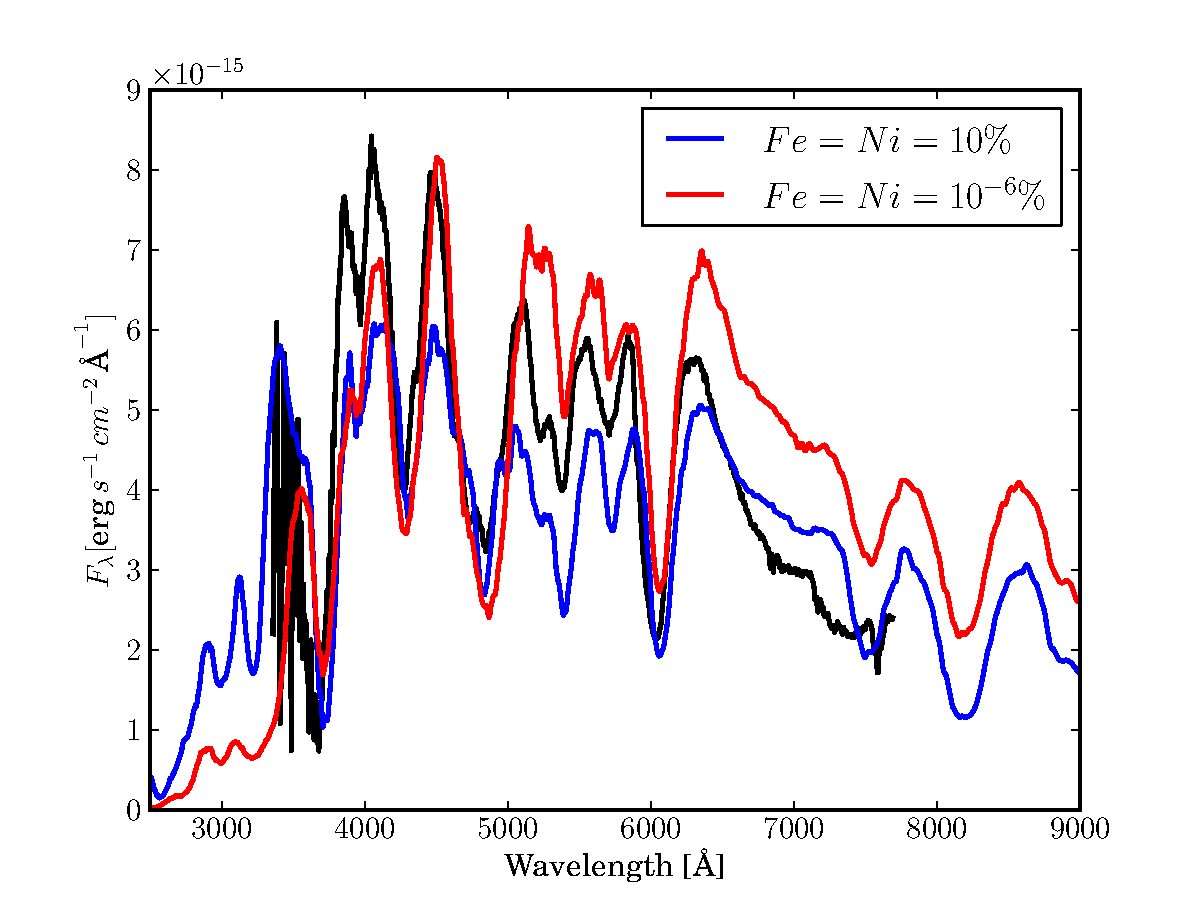
\includegraphics[width=0.7\textwidth]{chapter_dalek/plots/bf2002bo-10_ige.pdf} 
   \caption[Effect of iron group elements on MLMC fit]{When changing the \glsentryname{ige} (in this case we have only changed $\textrm{Fe}_0$ and $\textrm{Ni}_0$) the flux is altered in the blue and red part. Too much \glsentryname{ige}s and there's not enough flux in the blue and too much flux in the red and vice versa.}
   \label{fig:sn2002bo_ige_offset}
\end{figure}

There are six other abundances that are taken into account when fitting: carbon, oxygen, magnesium, silicon, sulphur and calcium (see Figure \ref{fig:sn2002bo_lineident}). Judging the fit of the \ion{Ca}{2} line at 3700\,\AA\ is relatively easy and thus the calcium abundance is usually changed first. An additional constrain on the calcium abundance is the \gls{nir} triplet near 8500\,\AA, which is however often missing in spectral coverage. The choice of temperature imposed by photospheric velocity and luminosity does not have an immense influence on this line. One caveat however is that the \ion{Ca}{2} line saturates at a certain abundance. If the observed \ion{Ca}{2} line is close to that limit one can only extract a lower limit for the calcium abundance.

Silicon and sulphur are usually the next elements to be fine-tuned. Both of these elements are linked through nuclear synthesis and we do not expect there to be more sulphur than silicon. We also expect no less sulphur than a third of silicon. Silicon also provides an important measure for temperature through the ionization balance, which is seen as the ratio between \ion{Si}{2} at 6150\,\AA\ versus the fit of \ion{Si}{2} at 5700\,\AA\ (see Figure \ref{fig:sn2002bo_vph_offset}). This effect was first mentioned in \cite{1995ApJ...455L.147N} and is explained in detail in \citep{2008MNRAS.389.1087H}. The strong \ion{Mg}{2} feature near 4300\,\AA\ helps constrains the magnesium abundance. The weak \ion{C}{2} feature at $\approx 6300\,\AA$ is the only line to provide constraints for the carbon abundance. In most \sneia\ spectra this line is weak or not visible and mainly provides an upper limit for the amount of carbon.

\begin{figure}[tb] %  figure placement: here, top, bottom, or page
   \centering
   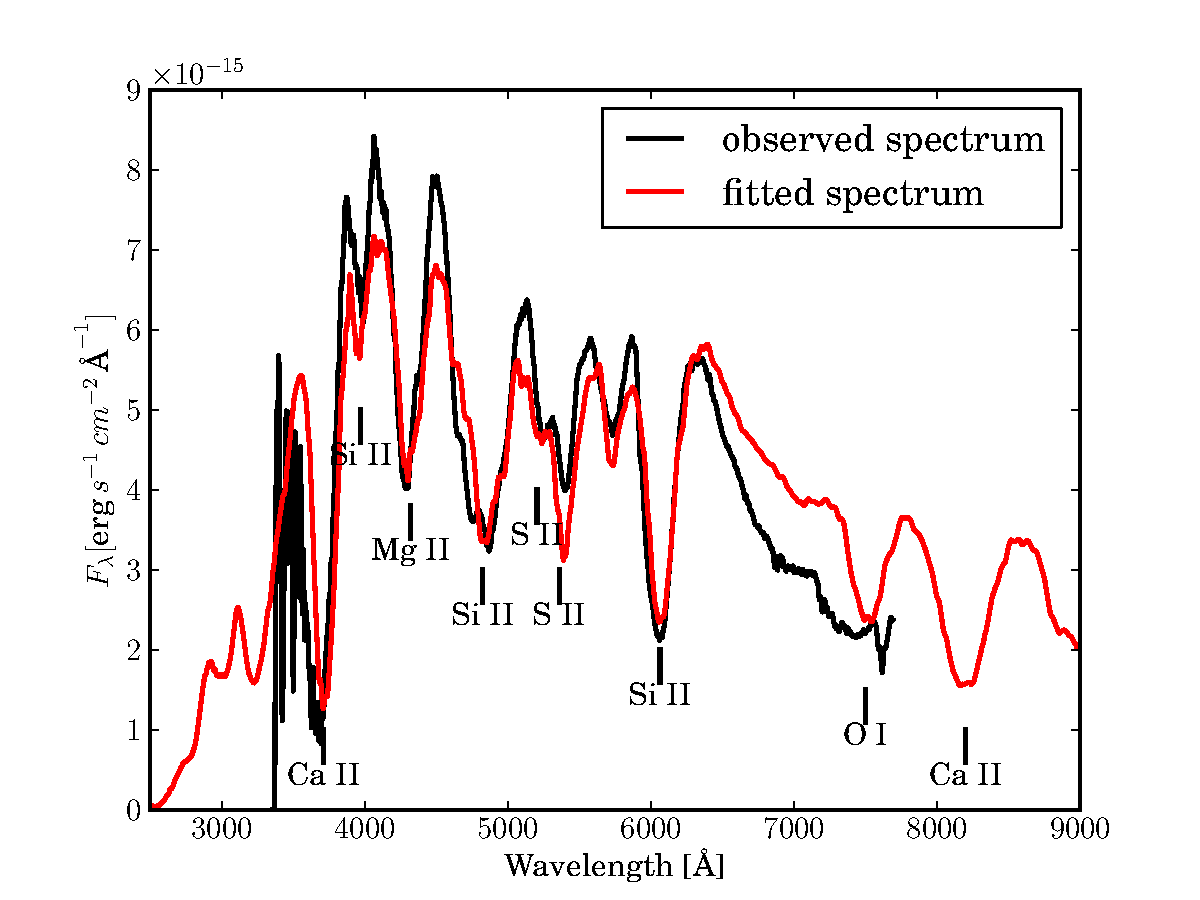
\includegraphics[width=0.7\textwidth]{chapter_dalek/plots/bf2002bo-10_lineid.pdf} 
   \caption[Best-Fit of SN 2002bo with MLMC including line identification]{The best-fit model for \sn{2002}{bo} We have identified some of the strongest lines that are scrutinized when fitting a \glsentryname{snia} spectrum.}
   \label{fig:sn2002bo_lineident}
\end{figure}

The last element to be described is oxygen, which takes the rest of the mass fraction when all other elements have been assigned abundance fractions. We will sometimes refer to this as a buffer element, but we caution the reader to not think of this as a physical description but rather a description of implementation. Such a buffer is needed as we have chosen a density distribution (\gls{w7}) and the elemental abundances are fractions by mass. Oxygen is chosen for that role as it does not have strong influence over the overall spectrum. Oxygen in general is not a major contributor to lines, the only strong lines are the \ion{O}{1} triplet at 7774\,\AA. This line is often very weak as a large fraction of oxygen is ionized and significant contamination from silicon and magnesium to the triplet. Both of these arguments mean that large fractions of oxygen might not be visible in the spectrum making it a perfect buffer element. 


The fitting process usually involves first adjusting luminosity, then \glspl{ige} and finally photospheric velocity. This is followed by adjusting the other elemental abundances from the initial values. After the elemental abundances are adjusted we re-adjust the luminosity, photospheric velocity and \gls{ige}. This iterative process continues until a satisfactory fit has been obtained. When closing in on the optimal fit we consider the dilution factor. Purely theoretical we would expect this to be close to 0.5 for a `physical' fit. We do, however, accept values between 0.4 and 0.7 as physical. This large range is accepted due to numerical fluctuation and approximations made by the \gls{mlc}. The parameters are often improved further by checking their time evolution through fits of photospheric spectra at different times.

\ctable[
caption = {Parameters for best fit},
	% 
	label   = {tab:2002bo_bestfit_abundances},
	%
	%
]{lcc}{
}{ \FL
% 
Parameter & Value & Realistic Constrains\ML
$\log{L/\lsun}$& 9.05&\\
\gls{vph}&11700&\\
Carbon & 0.08 \% &  C $<$ 12.5\,\%\\
Oxygen & 54.9 \% & C $<$ O \\
Magnesium & 10 \%&- \\
Silicon & 25 \% & Si $>$ 1\,\% \\
Sulphur & 4.5 \% & 1 $<$ Si/S-ratio $<$ 10\\
Calcium & 1 \% & Ca $<$ 5\,\%\\
Titanium & 0.01 \% &Ti + Cr $<$ 1\,\% \\
Chromium & 0.07 \% &Cr/Ni$_0$-ratio $<$ 10 \\
pre-existing Iron & 0.07 \%& Fe$_0$/Ni$_0$-ratio $<$ 10 \\
undecayed Nickel & 1.5 \% &$\textrm{Ni}_0$ $<$ 80\,\% \\
\LL}





Finally, during and after the fitting process the elemental abundances and ratios (listed in Table \ref{tab:2002bo_bestfit_abundances}) are also checked against theoretical nucleosynthetic yields \citep[e.g.][]{1999ApJS..125..439I}. If the abundances and abundance ratios are outside of these generous bounds one normally tries to find another reasonable fit within the bounds. We have also implemented this checking into our automatic optimization routines (see Section \ref{sec:dalek}).

In summary, the fit is relatively good as seen in Figure \ref{fig:sn2002bo_lineident}. There are however some problems that are intrinsic to the \gls{mlc} and can not be rectified by adjusting parameters. The calcium line at 3900\,\AA\ can be seen to be to blueshifted in relation to the model. This property is not unusual and is thought to come from high velocity calcium components at the outer edge of the ejecta. This can often be rectified in the stratified version of the \gls{mlc} which is not discussed in this work. The next major known discrepancy is the excess of flux redwards of  $\approx 6200\,\AA$.  This is a common problem rising assumption of an underlying black body spectrum, which overestimates the flux in this region. Although the continuum is offset we still believe the line depth to be representative, thus when fitting manually often one tries to fit the depth of the lines instead of the continuum. This excess makes it difficult to use traditional fitness measures and we will discuss the path we took in Section \ref{sec:dalek}.

In the end, the fitting of a supernova is a complex procedure and requires a lot of practice. For automating this process we initially tested simple gradient methods. These failed abysmally. We quickly discovered the search space is too complex and evaluation time takes too long (each synthetic spectrum roughly one minute on a modern computer) to use these simple methods. Research in numerical optimization techniques has made significant process in the last decades. These areas of mathematics have yielded impressive algorithms. Genetic algorithms are easy to implement and are intrinsically parallel. A perfect match for our problem.

\section{Brief Introduction to Genetic Algorithms}
\label{sec:ga_brief_intro}
Before advancing to the description of the automation of the \gls{mlc} we will give a brief introduction to \glspl{ga} which are used in the automation endeavour.   We urge the reader to review \glspl{ga} in Chapter \ref{chap:ga} before proceeding. 

The complexity of an optimization problem rises with the number of dimensions, but more so with the correlation of the input parameters. Iterative algorithms, often using gradients to find extrema by solving a Hessian matrix, are very good at problems with a low number of dimensions and small correlation between input parameters. They can exactly solve the problem in a very small amount of computational time. However as the search space gets more complex and multiple extrema start to appear. The iterative algorithm often converge on those and are only useful when starting close to the global optimum. For these complex multi-dimensional parameter spaces stochastic optimization techniques that rely heavily on random numbers are often the best choice. Unlike the iterative methods, however, stochastic optimization algorithms are not guaranteed to find any optimum. 

Automatically fitting \snia\ spectra is a very complex multi-dimensional parameter space with many highly correlated parameters. We have chosen \glspl{ga} - a stochastic optimization algorithm - to conquer this problem. \glspl{ga} use terminology which borrows from its roots in evolutionary science. At the core of each \gls{ga} is the \gls{individual}. The individual represents one solution in search space. The \gls{genotype} of the individual is the vector representation of all of its parameters, sometimes referred to as \gls{genome}. Evaluating the \gls{genotype} leads to the \gls{phenotype} which is the \gls{individual}'s representation in solution space (e.g. a spectrum obtained from parameters). For optimization one needs to have a quality measure which in terms of \glspl{ga} is the \gls{fitness}. The \gls{fitness} is calculated using a \gls{fitness} function from the \gls{phenotype} of the \gls{individual} (e.g. the $\chi^2$ value calculated for a synthetic spectrum against the observed spectrum).

\gls{ga} have a number (called population size; as a rule of thumb ten times the number of parameters) of these \glspl{individual} in a collection known as a population or generation. This enables them to probe multiple areas in search space simultaneously, which makes these algorithms intrinsically parallel. During the optimization process \glspl{ga} go through several stages first of which is the initialization of the first generation. The easiest is to draw random parameters from the parameter space (there are more advanced techniques which are described in Chapter \ref{chap:ga}). Once this first generation is populated with the required number of \glspl{individual} we evaluate their \glspl{phenotype} and then their \gls{fitness}. Once this step is complete we want to form the second generation out of the old generation. Chapter \ref{chap:ga} gives a very detailed overview over the different processes building a new population, we will here only describe one path. First we use a method of randomly choosing individuals that still favours more fit \glspl{individual} over less fit \glspl{individual}. Using this process we select two \glspl{individual} of the old population for mating. For the mating process we employ a technique called single-point \gls{crossover} to create a new individual. This means that we select a random point in the \gls{genome} of both parents. Parameters before this point are taken from the first parent, parameters after that point are taken from the second parent. This newly created \gls{individual} (or \gls{child}) is then subjected to possible mutation, where each parameter has a small chance of being multiplied by a random number. We repeat this process of choosing two parents and creating children until the new generation has the same number of individuals as the old population. One should note that in this process it is possible, unlike in nature, that the parents are the same individual twice. This case normally only happens when the parent is very fit and chosen twice consecutively in a random process. The \gls{crossover} in this case does not change the child but creates a copy of the parent, which is then however subjected to mutation. 


To visualize this process we have created a flowchart in Figure \ref{fig:ga_overview}. This process of the creation of a new generation and subsequent evaluation is repeated until either a whole generation or an \gls{individual} has reached a certain threshold in \gls{fitness}. \glspl{ga} are relatively resistent to converging on local optima, but are not entirely immune to it. The convergence to a local optimum in \gls{ga} terms is called premature convergence. 

In summary, we have chosen \glspl{ga} because they are known to be able to navigate in complex search spaces. In addition they are inherently parallelizable which makes it easy to speed up the optimization routine. For a more detailed overview we urge the reader again to consult Chapter \ref{chap:ga}.

\begin{figure}[htbp] %  figure placement: here, top, bottom, or page
   \centering
   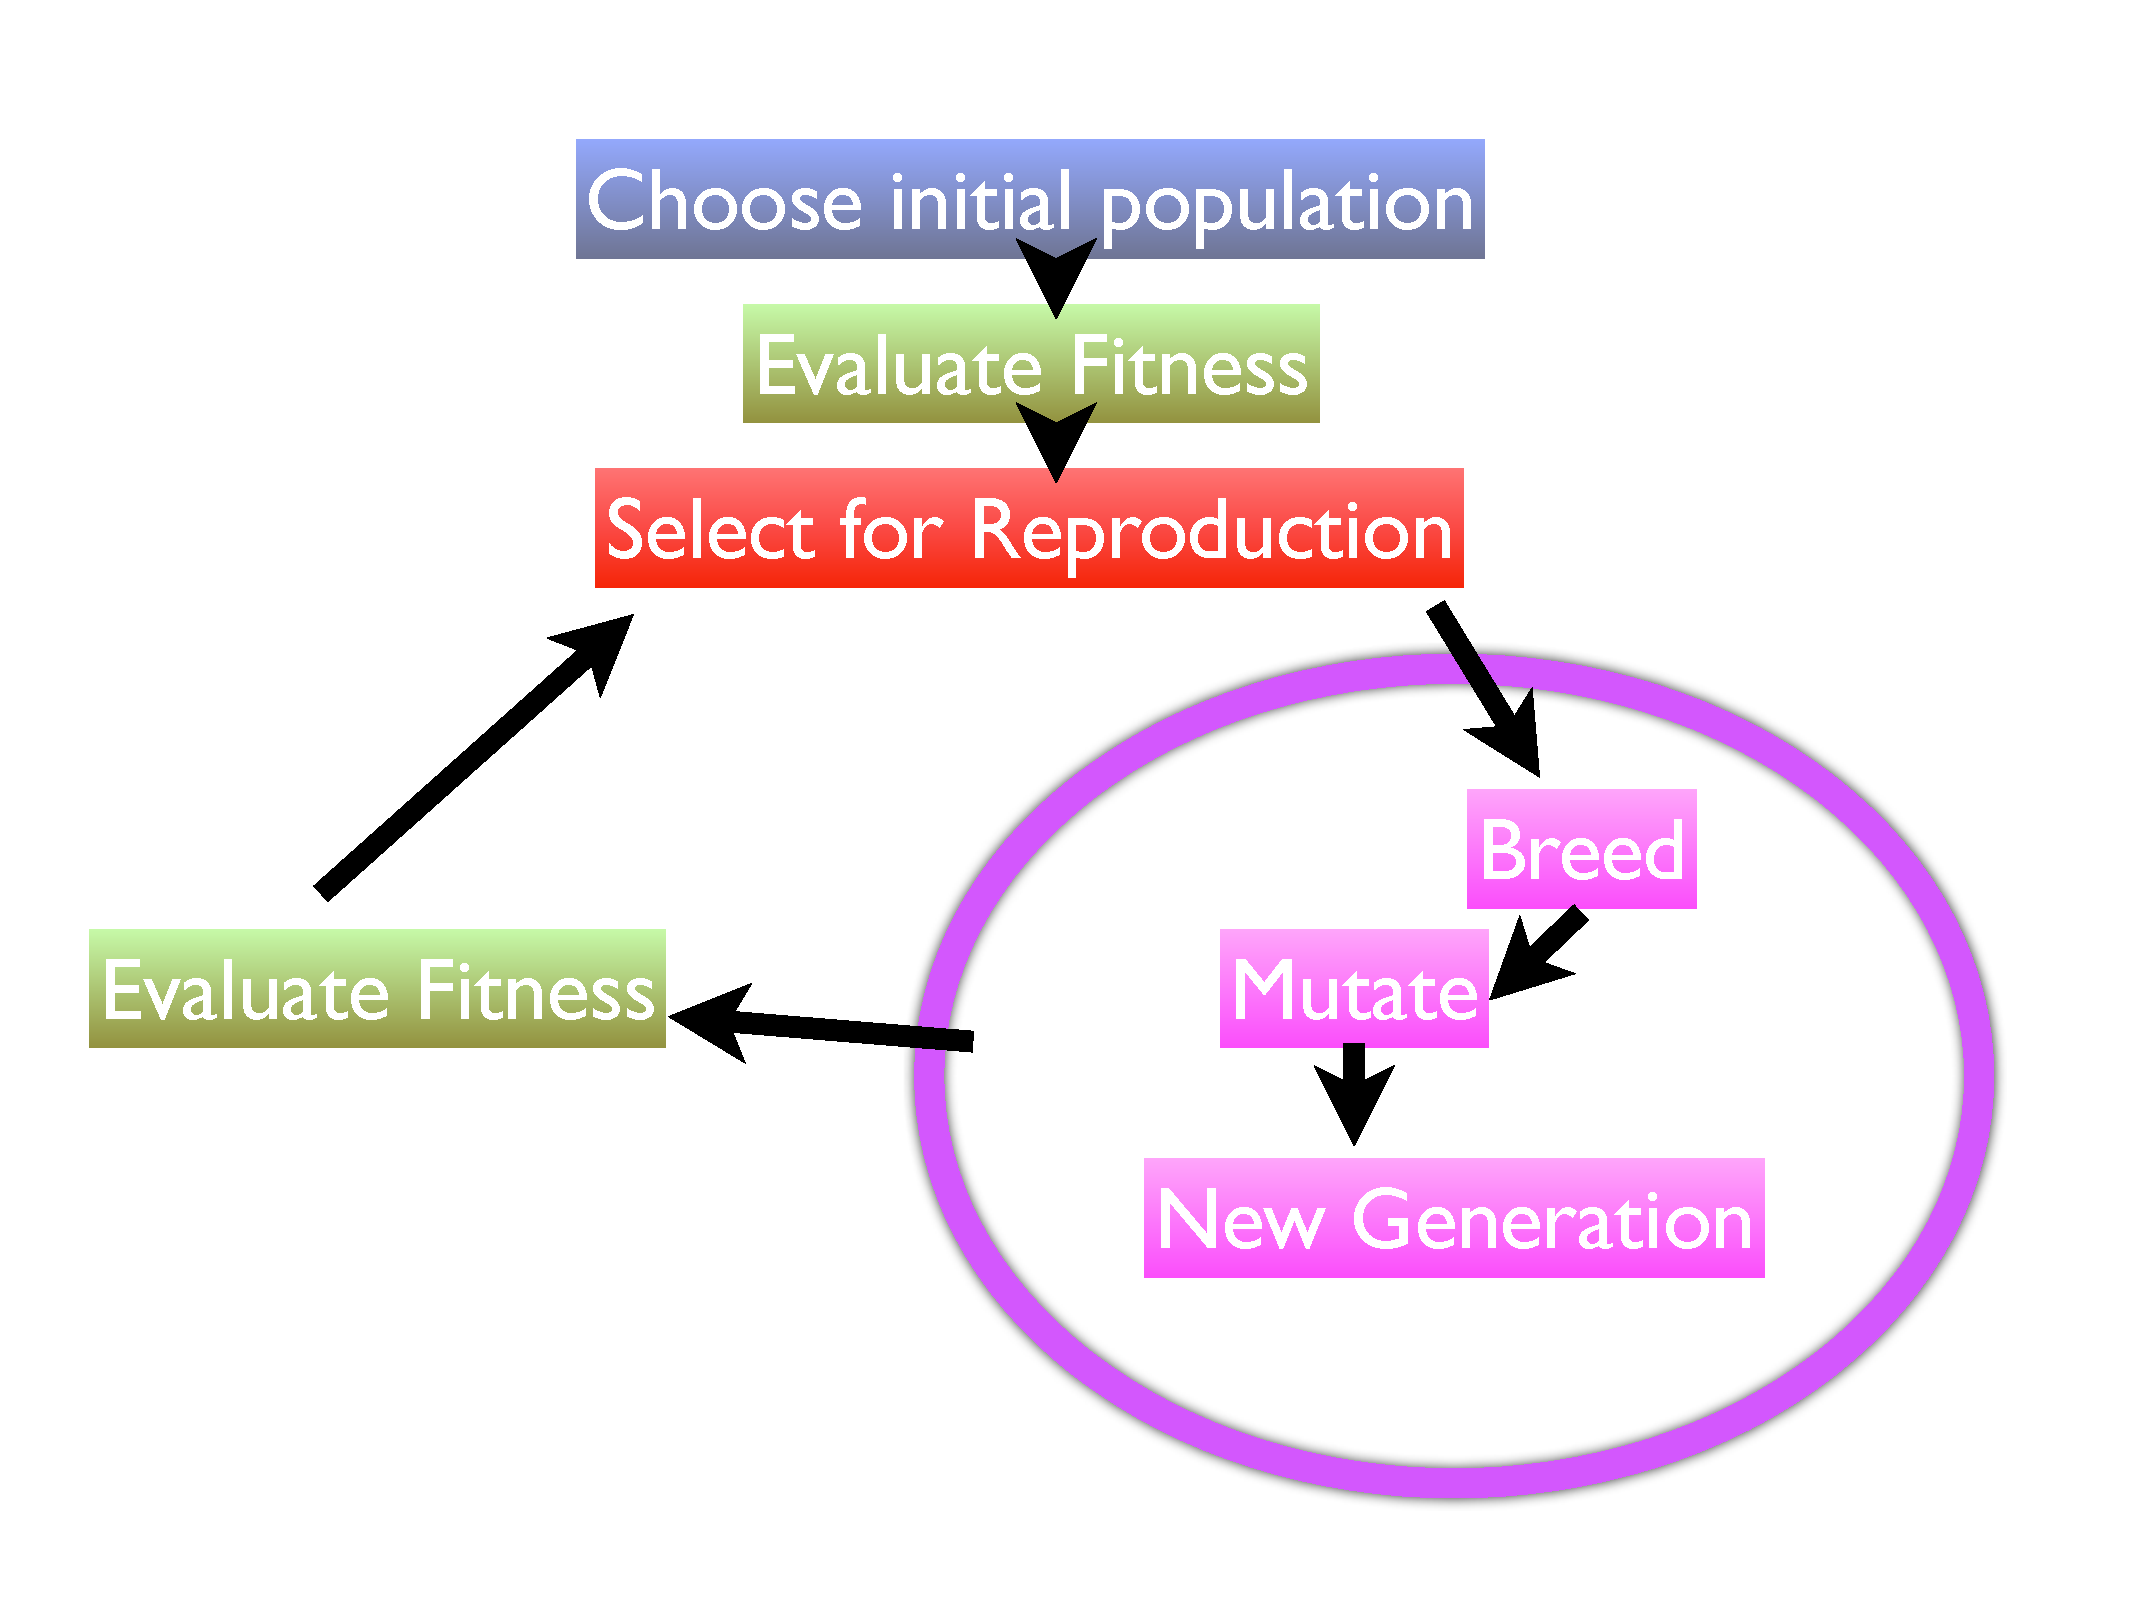
\includegraphics[width=0.7\textwidth]{chapter_dalek/plots/ga_overview.pdf} 
   \caption{Flow chart overview over the process of a \glsentryname{ga}}
   \label{fig:ga_overview}
\end{figure}



\section{Genetic Algorithms fit Type Ia Supernovae: The Dalek Code}
\label{sec:dalek}

In the following section I will outline the current progress of the automation of fitting the \sneia\ spectra with the \gls{mlc}. The torrent of new spectra observed by a multitude of surveys requires the swift and self consistent analysis of many \sneia\ spectra in a short time. As described in Section \ref{sec:manual_sneia} the search-space for fitting \sneia\ spectra is very complex and vast. It thus requires a smart and quick algorithm for analysis.

The parameters that need to be fit are luminosity, photospheric velocity (\gls{vph}), carbon, magnesium, silicon, sulphur, calcium, chromium and nickel prior to decay ($\textrm{Ni}_0$) as well as stable iron ($\textrm{Fe}_0$). As in the manual fitting example the time since explosion as well as the luminosity distance (for scaling purposes) are given. We initially tried a Newton-Raphson approach with multiple phases. In the first phase the algorithm would adjust luminosity and normally came close to the optimum. In a second phase we tried to let the algorithm re-adjust luminosity, then photospheric velocity and last \gls{ige} s. This was modelled after the manual approach that is taken by \citet{hachinger_dipl2007} and \citep{hachinger_phd2011}. The process was time consuming and did not readily converge. We realized quickly the search space is far to complicated for such simple methods. In addition, we were limited to one processor with the Newton-Raphson-like method and could not utilize the large number of multi-processor machines that are currently available. \glspl{ga} seem the perfect choice for this problem, as they are intrinsically parallel, are easy to implement and are relatively immune to local optima.

The first task was to wrap the \gls{mlc} code so that it is able to easily interface with any optimization routine and run in parallel in multiple instances. The initial version of this \emph{launcher} code was able to run on multiple processors on one machine. Next we extended the \emph{launcher} code to be able to distribute jobs on the network. As the institute has a heterogeneous computer structure (different processor types, different operating systems) we were forced to write a custom software to distribute it among the many nodes. An additional advantage to this cloud-like process structure is that we could use unused resources as well as avoid servers that are heavily demanded by other users. For the scheduling we used a simple first in, first out queue. Finally, the \emph{launcher} code has a simple \gls{api} that accepts arrays with parameter sets and returns the results in a simple array format. Invisibly to the user, it writes the parameter sets to the relevant disks in a format that the \gls{mlc} understands. Upon completion it reads the data files and cleans up any temporary files created by the \gls{mlc}. This abstraction of the \gls{mlc} allowed us to quickly explore the intricacies of the \glspl{ga} (and in the future possibly other optimization algorithms).


As described in Section \ref{sec:ga_brief_intro} the first step for any \gls{ga} is to create an initial population (first generation). One can easily draw uniform randomly for luminosity and \gls{vph} (within some bounds). However, this method does not work for the elemental abundances as the sum of the abundances needs to add up to one. As explained previously these abundances are abundances by mass with a pre-chosen \gls{w7} density structure. A population that is distributed around the optimum value converges much quicker than a uniformly sampled one. Thus we have chosen to use the \gls{w7} abundances as an input parameter as it seems to be a good starting point for many \snia. To calculate these abundances we need to know the photospheric velocity. Using data from \citet{2005ApJ...623.1011B} we have estimated an empirical relationship between the time since explosion and the photospheric velocity (see Figure \ref{fig:texp_vph}). This will serve as a rough first guess.

\begin{figure}[htbp] %  figure placement: here, top, bottom, or page
   \centering
   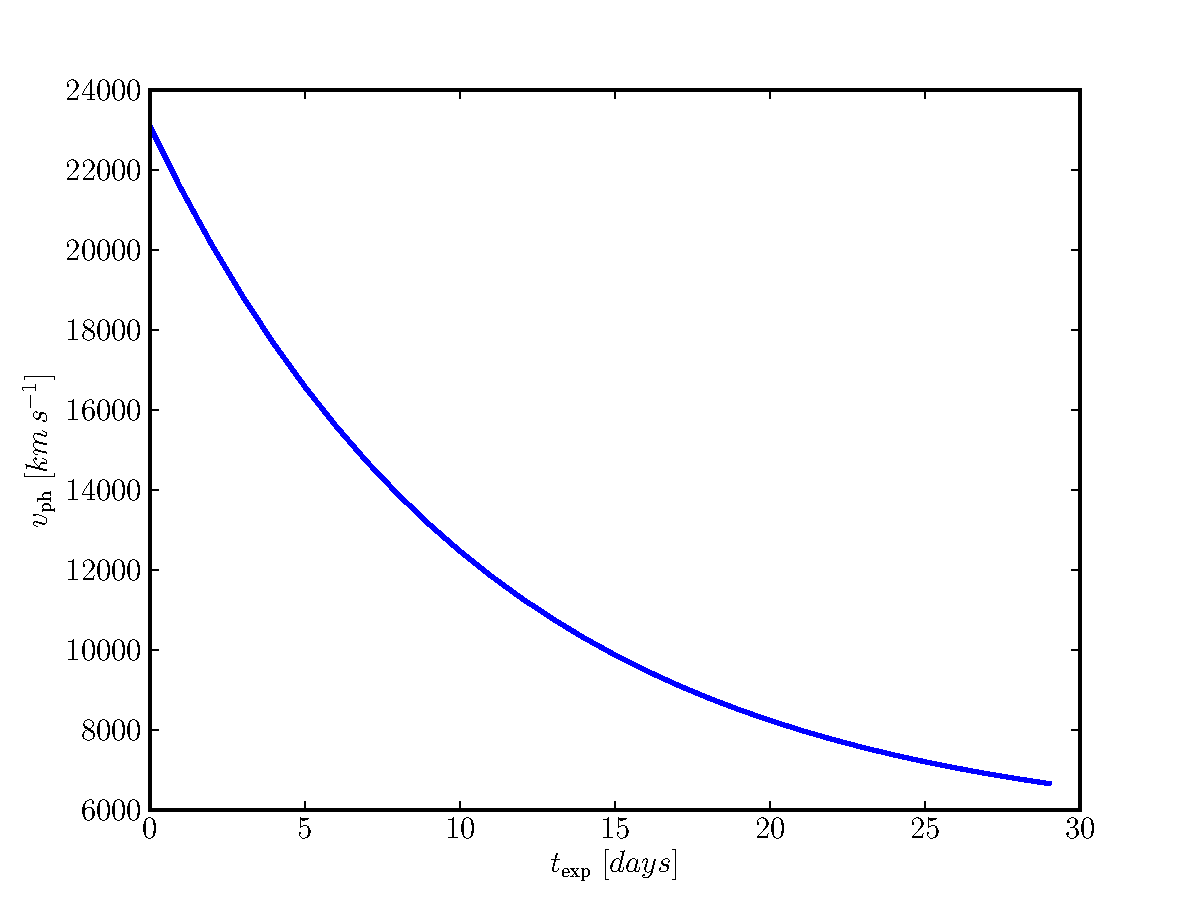
\includegraphics[width=0.7\textwidth]{chapter_dalek/plots/plot_texp_vph.pdf} 
   \caption[Estimated initial guess for photospheric velocity against days after explosion]{Estimated initial guess for photospheric velocity against days after explosion \citep{2005ApJ...623.1011B}. }
   \label{fig:texp_vph}
\end{figure} 

Once we know a \gls{vph}-estimate we can determine at what depth the photosphere is located in the \gls{w7}. We use this point and integrate outwards to find our initial abundance fractions.

When creating our initial population, we draw randomly from a uniform distribution for a preselected luminosity range (for the moment determined manually) and a \gls{vph} range 4000\,\kms above and below the \gls{vph} estimate. The random sampling of the elements poses some problems.There are a lower and an upper bound when it comes to the initial abundance ratios. We have a lower bound for each abundance (established as the smallest abundance an element can have by \gls{mlc}) at $10^{-7}$ and a upper bound which is determined by the requirement that all abundances need to add up to one. Knowing the minimum and maximum bound we then use a log-normal asymmetric random distribution around the actual \gls{w7} value with the lower and upper bound being at three sigma. If we would draw the abundances every time in the same order it would mean that the last element to be drawn would always have a very low chance of obtaining a high abundance value. Thus we randomize the order of drawing the elemental abundances. This ensures that the initial population is sufficiently dispersed to avoid the \gls{ga}'s premature convergence on a local optimum, but close enough to the region of interesting parameter space, which avoids unnecessary delay in the convergence. 

After creating an individual through the random drawing process, we also check abundance ratios allowed by explosive nucleosynthesis of a \gls{cowd} outlined in Table \ref{tab:2002bo_bestfit_abundances}. If the newly created individual does not conform with the abundance limits laid out in Table \ref{tab:2002bo_bestfit_abundances} it is discarded and a new one is drawn. Once the initial population (we chose 150 for our population size) is created it is distributed among the compute nodes by the \emph{launcher} module of the \gls{dalek}.

The resulting spectra are then subjected to a fitness function. The selection of the fitness function is one of the most crucial choices for any \gls{ga}. The correct fitness function is still a field of active research in the \gls{dalek}. As an initial approach we calculated the mean-square of the residuals remaining from subtracting the observed spectrum and the spectrum of the current individual. 

This approach has two main issues. First for almost all observed spectra in the early phase the fitted spectrum has a large continuum excess beyond 6500\,\AA (see Figure \ref{fig:sn2002bo-10_bf}). However, we still regard the line depth and line shape to be correct. As described previously this is a known issue of the \gls{mlc} code. This large difference in the infrared means that the \gls{dalek} will try to optimize this large offset and pay less regard to a good fit in the rest of the spectrum. To alleviate this we have tried multiple approaches. At first we tried to de-weight the fit in the problematic region. This artificially introduced weighting factor introduces another parameter which might have to change it for the \gls{ga} to succeed on different spectra. This would defeat the point of an automatic fit. As a second approach we tried to fit and subtract the continuum in the problematic region before creating our fitness figure. 

Secondly there are different parameters, including the dilution factor, that help guide the fit which are neglected when just using the traditional mean-square approach. For example, the dilution factor is expected to be close to 0.5 (see description in Section \ref{sec:mlc_intro}). \citet{hachinger_dipl2007} and \citet{hachinger_phd2011} have found that in all cases a good fit will have a value of the dilution factor between 0.4 and 0.7. We have incorporated this into the fitness calculation and de-weight the fitness of spectra with a value outside this range to a great extent. Due to both these reasons, we now include a traditional goodness of fit measure in the blue, the more complex fitness calculation described above and an inclusion of the dilution factor $W$ in the final fitness.

We should mention that we have tried, in addition to calculating the root-mean-square of the spectral fit, a number of completely different methods. Most notably we tried to use neural networks to perform a goodness of fit analysis. We however abandoned this effort as the training set to calibrate neural networks requires a large number of well fitted spectra which are not available. 

Once the fitness is calculated for each individual we use the method of fitness scaling to preempt premature convergence in early generations (caused by the so called `super-individuals') as well as creating a steeper fitness gradient in later generations. We have decided to use a linear fitness scaling as described in \citet[see page 76 of]{citeulike:125978}:
\[
f^\prime = af+b,
\]
where $f\prime$ designates the scaled fitness and $f$ the raw fitness.
In all cases we want to make sure that the average of the scaled fitness $f_\textrm{avg}^\prime$ equals that of the average of the raw fitness $f_\textrm{avg}$. We will first try to find a linear relation so that the new maximum fitness $f'_\textrm{max}$ is $C_\textrm{mult}$ times the average fitness ($f_\textrm{avg}$). We choose $C_\textrm{mult}=2$ as suggested by \citet{citeulike:125978}. This operation will scale early `super-individuals' down and the rest of the population up and preempts premature convergence. In the later phases of the \gls{ga}, when the fittest individuals and the bulk of the population have similar fitness values, this operation would lead to negative fitness values for some individuals. In that case we find a scaling parameters that maps the least fit individual to a fitness value of 0, while still maintaining $f_\textrm{avg}^\prime=f_\textrm{avg}$. Once we have scaled the fitnesses we move to the selection process.

In the current version of the \gls{dalek} we employ \textit{elitism} (10\% of fittest individuals advance immediately to next generation). We have also experimented with other modifications to the mating population, but found them to be subpar. The mating pool we have chosen has only two slots. For now we select the individuals for the mating pool using the standard \gls{rws}. 

We use a \gls{crossover} probability of 90\%, this means that in 10\% of the cases we do not perform \gls{crossover}. This means that the child is a copy of the first parent. If \gls{crossover} occurs, we perform a uniform crossover as we felt that we do not want the ordering of the parameters to matter. We have also experimented with arithmetic \glspl{crossover} by taking the mean of the parents. This meant that often useful traits would entirely disappear and we switched back to uniform \glspl{crossover}. We will experiment in the near future with different crossover techniques like single-point \glspl{crossover}. 

The new individual, created by crossover, is subjected to possible mutations before being placed into the new population. The \gls{dalek} employs different mutation strategies for the different parameters. The abundances are just multiplied by a uniform random number (we have tried gaussian random numbers, but this led to premature convergence in many cases) with a relatively high chance of currently 7\%. Luminosity and photospheric velocity are physically different from the element abundances and as such are treated differently in the mutation process. In both cases we add a uniform random number, in addition to having different mutation probabilities (this applies to all elements but oxygen). After the mutation step we see if the buffer element oxygen has a negative abundance. A negative abundance implies that the other elements add up to more than one. If oxygen has positive abundance the code goes on to check the abundance ratios. If the child passes both these tests it is placed in the new population, if not it is discarded. This process is repeated until the size of the new population (including the members of the old population that advanced through \textit{elitism}) reaches 150.

This process of selection, recombination and mutation is repeated over many generations. We have experimented with up to a 1000 generations in one run. Our scheduler can achieve a throughput of one generation per minute (in optimal conditions where all CPUs are free). 
Our principal spectrum for testing the \gls{ga} was \sn{2002}{bo} 10.4 days post explosion (see Figure \ref{fig:sn2002bo-10_bf}). We have also tried different spectra with varying degree of success.

In the presented case we let the \gls{ga} run for 188 generations. Figure \ref{fig:fitness_evolution} shows how the genetic algorithm over many generations improves the fitness of the \glspl{individual}. 

\begin{figure}[tb] %  figure placement: here, top, bottom, or page
   \centering
   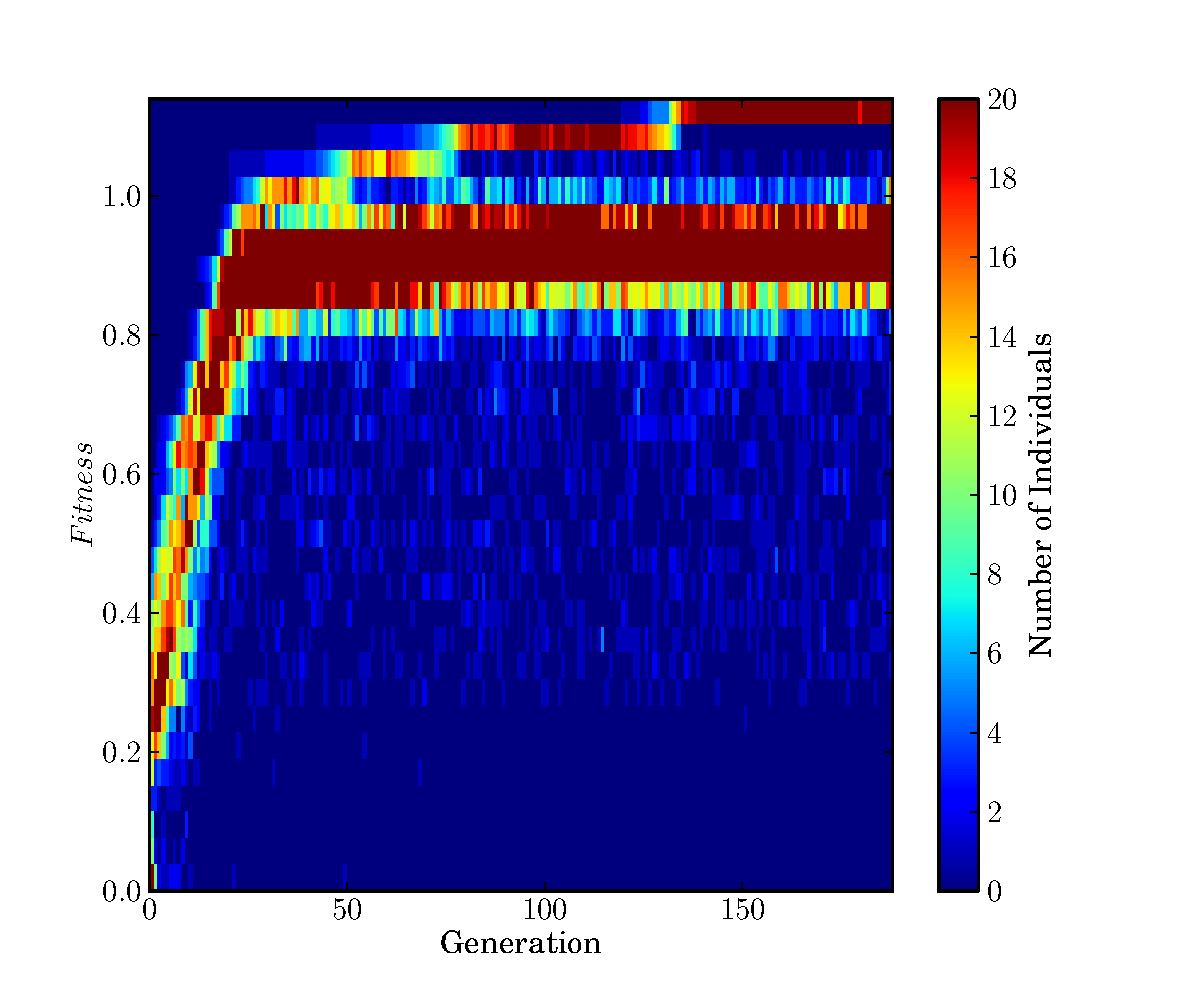
\includegraphics[width=0.7\textwidth]{chapter_dalek/plots/plot_02bo_fit_evol.pdf} 
     \caption[Evolution of fitness over the generations]{Evolution of fitness over the generations. In later generations there is a clear divide between the members that have advanced through elitism and the bulk of the population. This suggests a too high mutationrate or the convergence of the algorithm. }
   \label{fig:fitness_evolution}
\end{figure}

The step-pattern is very common in genetic algorithms: One individual has a favorable mutation and it takes several generations for the other \glspl{individual} to catch up. During the last generations one can clearly see that there is a gap between the bulk of the population and the top 10\%. This gap is caused by the contrast of relatively high mutation in the main individuals against the mutation free advancement of the top 10\% (\gls{elitism}).


\begin{figure}[tb] %  figure placement: here, top, bottom, or page
   \centering
   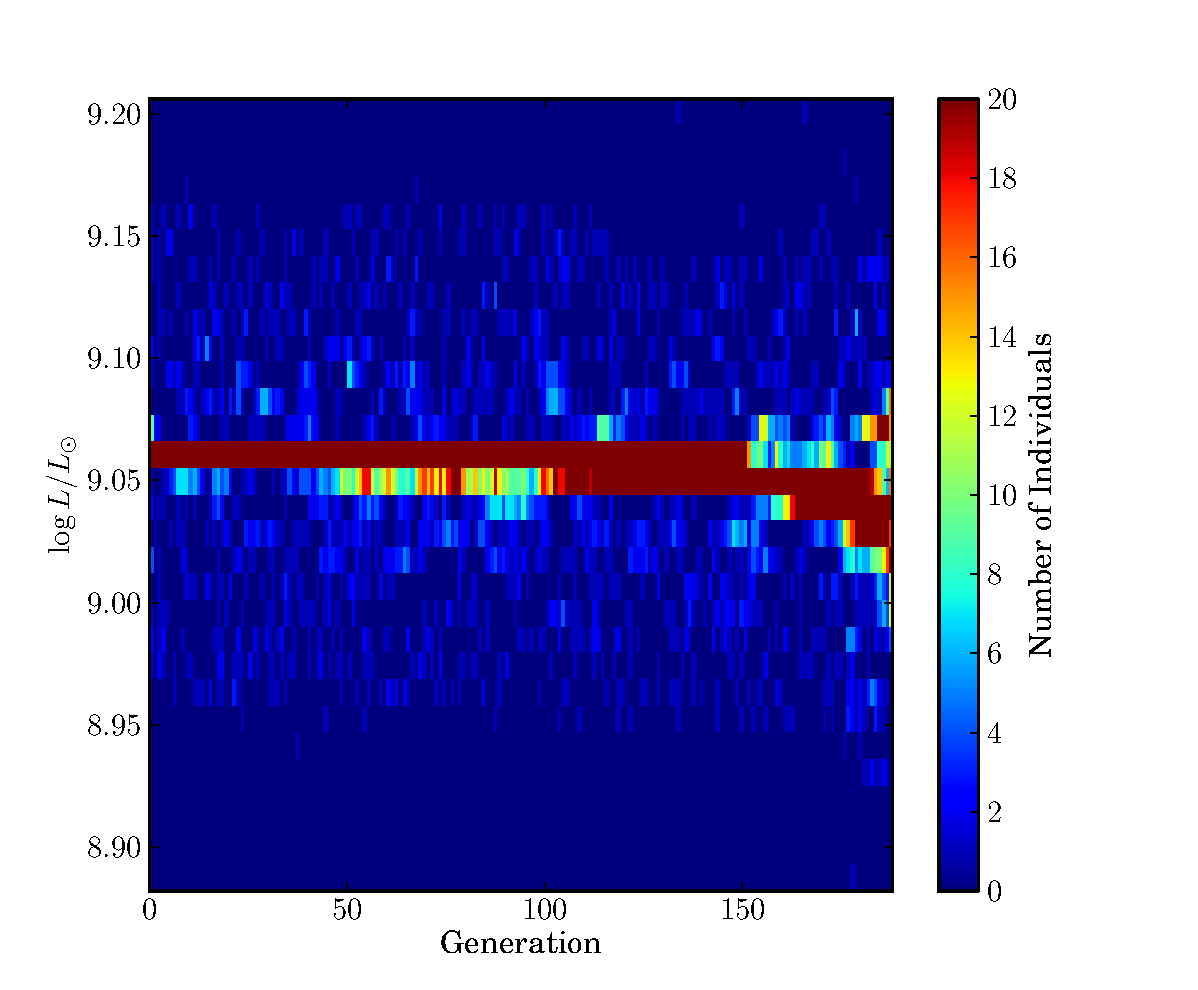
\includegraphics[width=0.49\textwidth]{chapter_dalek/plots/plot_02bo_lum_evol.pdf} 
   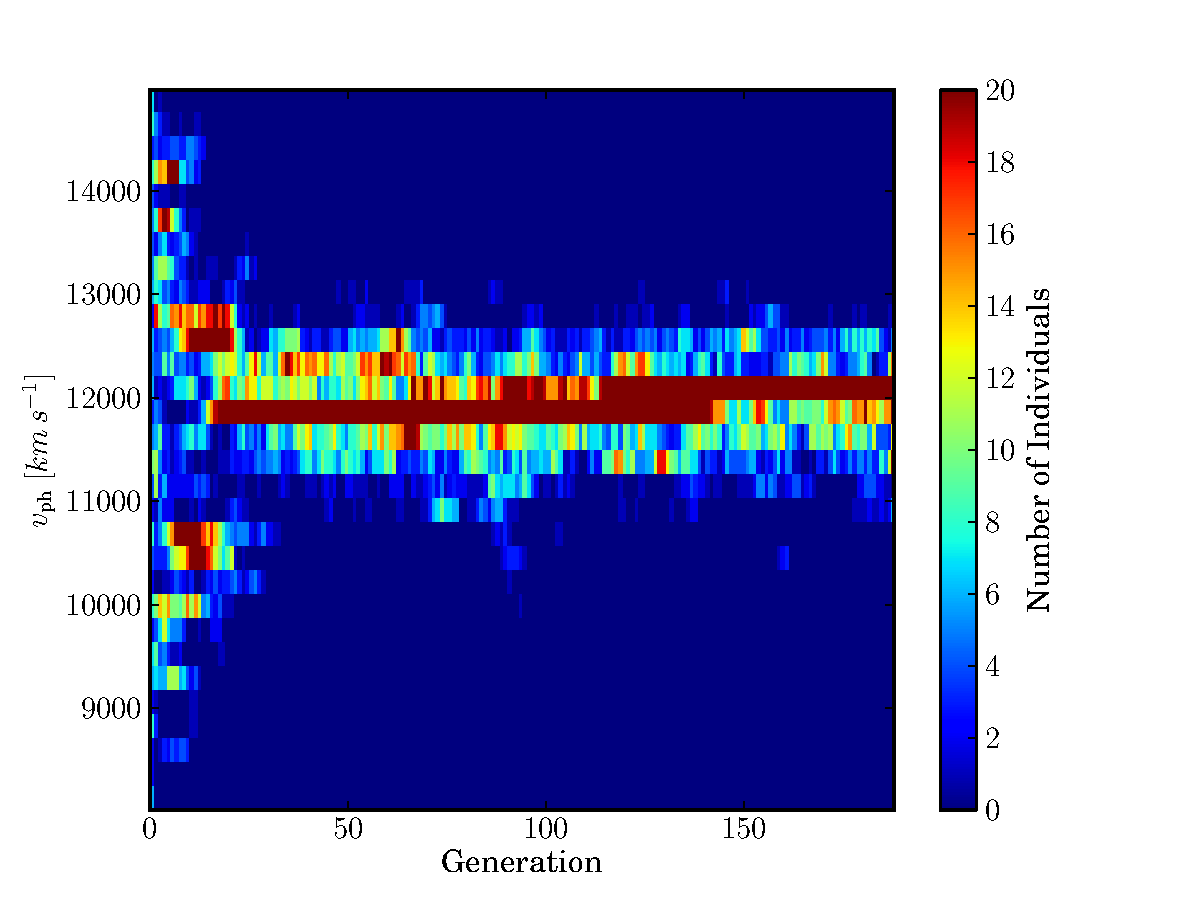
\includegraphics[width=0.49\textwidth]{chapter_dalek/plots/plot_02bo_vph_evol.pdf} 
   \caption[Evolution of both luminosity and photospheric velocity over generations]{The evolution of both luminosity and photospheric velocity shows that even at late phases of the algorithm there are still new combination that are being trialled. The very quick convergence in both cases however is a bit worrisome and will be analysed in future experiments.}
   \label{fig:lumvph_evolution}
\end{figure}


Figure \ref{fig:lumvph_evolution} gives a good overview of how the genetic algorithm wanders through the parameter space. In our example the algorithm converges relatively fast (after roughly 30 generations). Even though there is a `main'-population the algorithm still tries out different combinations. Currently we still have the problem that for certain initial random seeds the algorithm does not find the global optimum but converges prematurely on a local optimum. We believe the quick convergence seen in Figure \ref{fig:lumvph_evolution} might be evidence for this. This again is an area of active research and two experts in evolutionary optimization joined our team recently to address this problem. 

\begin{figure}[tb] %  figure placement: here, top, bottom, or page
   \centering
   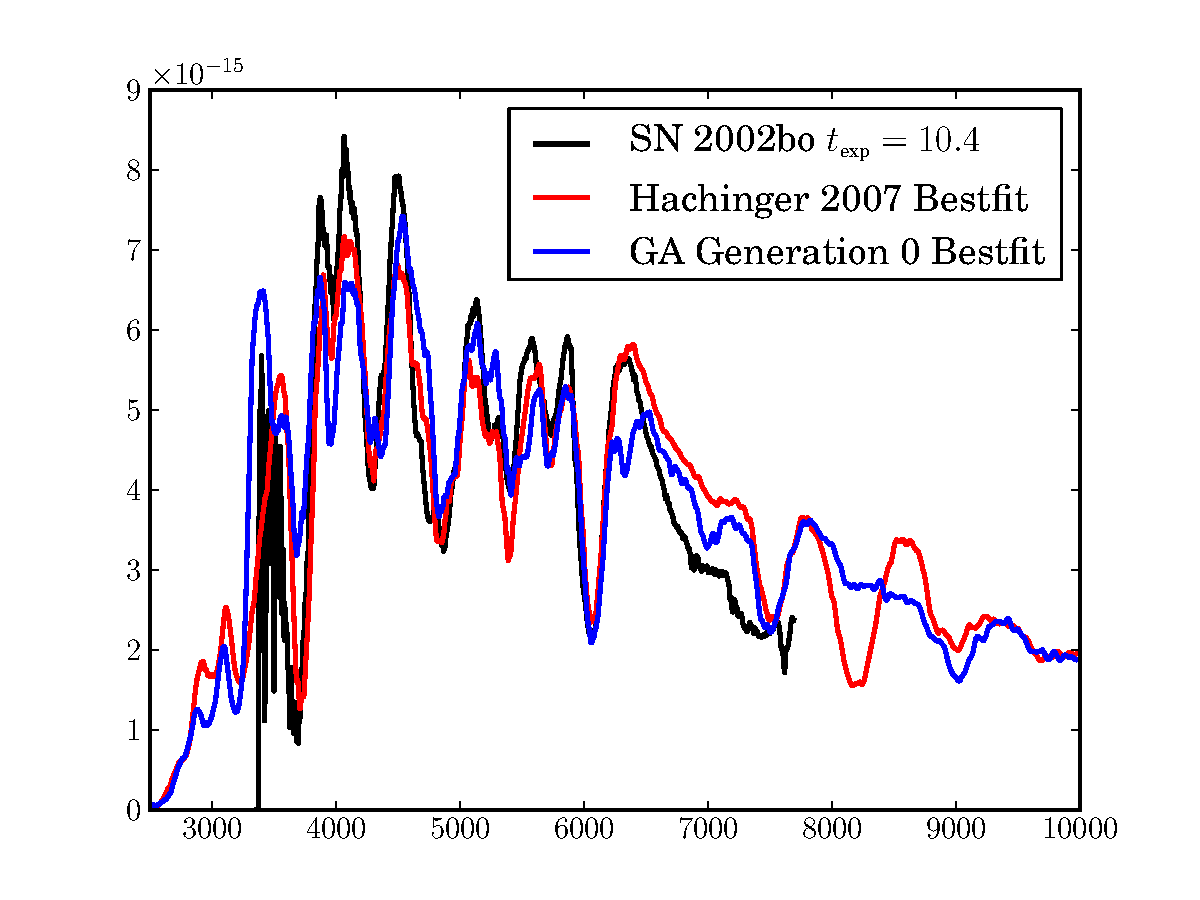
\includegraphics[width=0.49\textwidth]{chapter_dalek/plots/plot_ga0_speccompare.pdf} 
   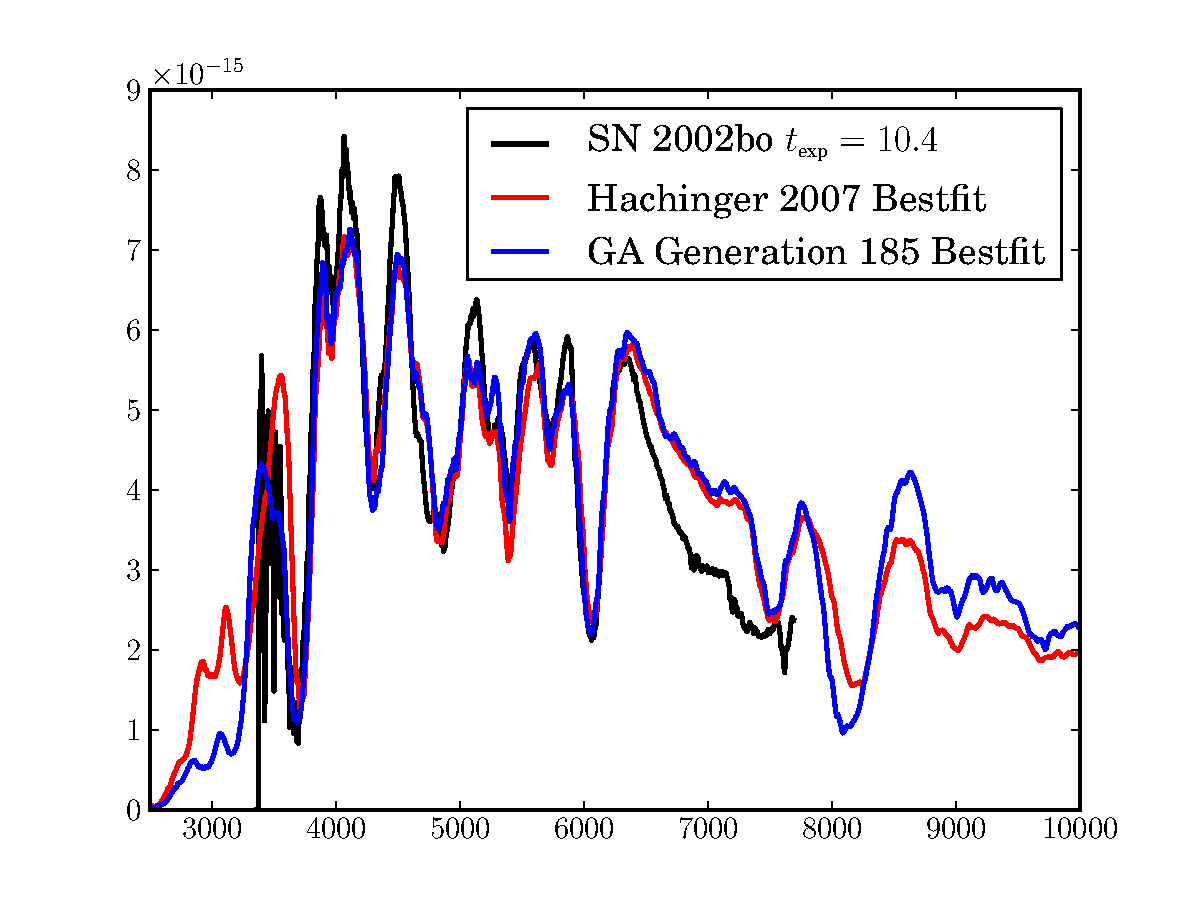
\includegraphics[width=0.49\textwidth]{chapter_dalek/plots/plot_ga185_speccompare.pdf} 
   \caption[Results of optimizations with Genetic Algorithms]{The best individual of the first generation (left) and the best individual after 185 generations (right). This initial result demonstrates that \glsentryplural{ga} are able to conquer this problem. A more stable convergence and thorough exploration of the parameter space is however necessary to use this technique on a set of supernova spectra.}
   \label{fig:example}
\end{figure}

Although there are still many outstanding problems we can show that the \glspl{ga} are able to solve the \sneia\ fitting problem. In Figure \ref{fig:ga_fit} we show the best fit in the first generation as well as the best-fit in the last generation. As comparison we show the best fit obtained by \citet{hachinger_dipl2007}. The \gls{ga} has been successful in reproducing the main features of the \sneia-spectrum. The de-weighting in the infrared is working very well. Finally, we are currently trialing the \gls{dalek} on different spectra with mixed results. 


\section{Conclusion}
\label{sec:dalek_conclusion}


We have completed two major steps for the automation of \sneia\ fitting. First we have written an easy \gls{api} that allows many synthetic spectra to be created simultaneously on an array of machines. Secondly we have demonstrated that \gls{ga} are powerful tools which can find solutions efficiently in the vast parameter space of \sneia\ spectra. We do acknowledge that our current implementation does not reliably work on all spectra and there remains lots of fine-tuning work to be done. This tweaking is very common in \gls{ga} implementations, but often requires experts in numerical optimization for speedy advancement. James Montgomery and Irene Moser are experts in evolutionary optimization (their research focuses on differential evolutionary algorithms) and are currently exploring with our help the search space. 

Once the \gls{dalek} is able to fit spectra reliably with the current code we plan to first use this on a large set of \sneia\ spectra and explore general abundance trends. Similar to \citet{2007Sci...315..825M} we plan to unravel the stratification and mass of the ejecta. Depending on the explosion mechanism (deflagration or detonation) we will find different elemental abundances. Either explosion mechanism will likely hint at the mass of the white dwarf just prior to explosion. This will be an important indicator for the still unsolved progenitor question addressed in the other chapters of this thesis. Finally, we will plan to extend the \gls{dalek} to use the stratified version of the \gls{mlc}, while much more complicated,  will help us to improve the models of the layered structure of \snia.

On a different front we are also exploring ways to optimize the parameter space exploration speed. Even on current high-end machines the \gls{mlc} takes one minute per synthetic spectrum per CPU. One of the ideas is creating a parameter grid around all or some of our search area. We could then use fast and efficient interpolation techniques (one of these is described in Chapter \ref{chap:ndinterp}) and explore different settings for our genetic algorithm much more quickly.

Over the course of this project we have realized that the field of numerical optimization has made huge strides in the last decades. Most of the new algorithms are not well known in astronomy and are used even rarer. On the other hand experts in the field of numerical optimization are often in desperate need for `real world' applications. They are more than willing to apply their knowledge to problems in our field. We strongly believe that there is an important ground for collaboration that would benefit both sides immensely.





